\begin{frame}
	\textbf{Econometric Problems}
	\begin{itemize}\setlength\itemsep{1em}
		\item \textbf{Evaluation Problem} We only observe an individual's wage in the sector they are working in.
		\item \textbf{Selection Problem} As individuals pursue their comparative advantage, we only observe selected samples from the latent skill distribution in either sector.
	\end{itemize}\vspace{0.5cm}
\end{frame}
%-------------------------------------------------------------------------------
%-------------------------------------------------------------------------------
\begin{frame}
	\textbf{Key Questions}\medskip
	\begin{itemize}\setlength\itemsep{1em}
		\item What economic concepts are accounted for, which are not?
		\item What does the individual, what does the econometrician know?
		\item What gives rise to heterogeneity in skills?
	\end{itemize}
\end{frame}
%-------------------------------------------------------------------------------
%-------------------------------------------------------------------------------
\begin{frame}
	\begin{itemize}\setlength\itemsep{1em}
		\item Skills follow a bivariate normal distribution denoted by $F(s_1, s_2)$.
	\end{itemize}	
	\begin{align*}
	\begin{pmatrix}
	\ln S_1 \\
	\ln S_2
	\end{pmatrix}  \sim \mathcal{N} \left(
	\begin{pmatrix}
	\mu_1 \\
	\mu_2
	\end{pmatrix} , \begin{pmatrix}
	\sigma_{11}  &  \sigma_{12} \\
	\sigma_{21}&  \sigma_{22}
	\end{pmatrix} \right)
	\end{align*}
\end{frame}
%-------------------------------------------------------------------------------
%-------------------------------------------------------------------------------
\begin{frame}
	\begin{figure}[htp]\centering
		\caption{Joint Distribution of Skills}\label{Joint Distribution of Skills}\scalebox{0.35}{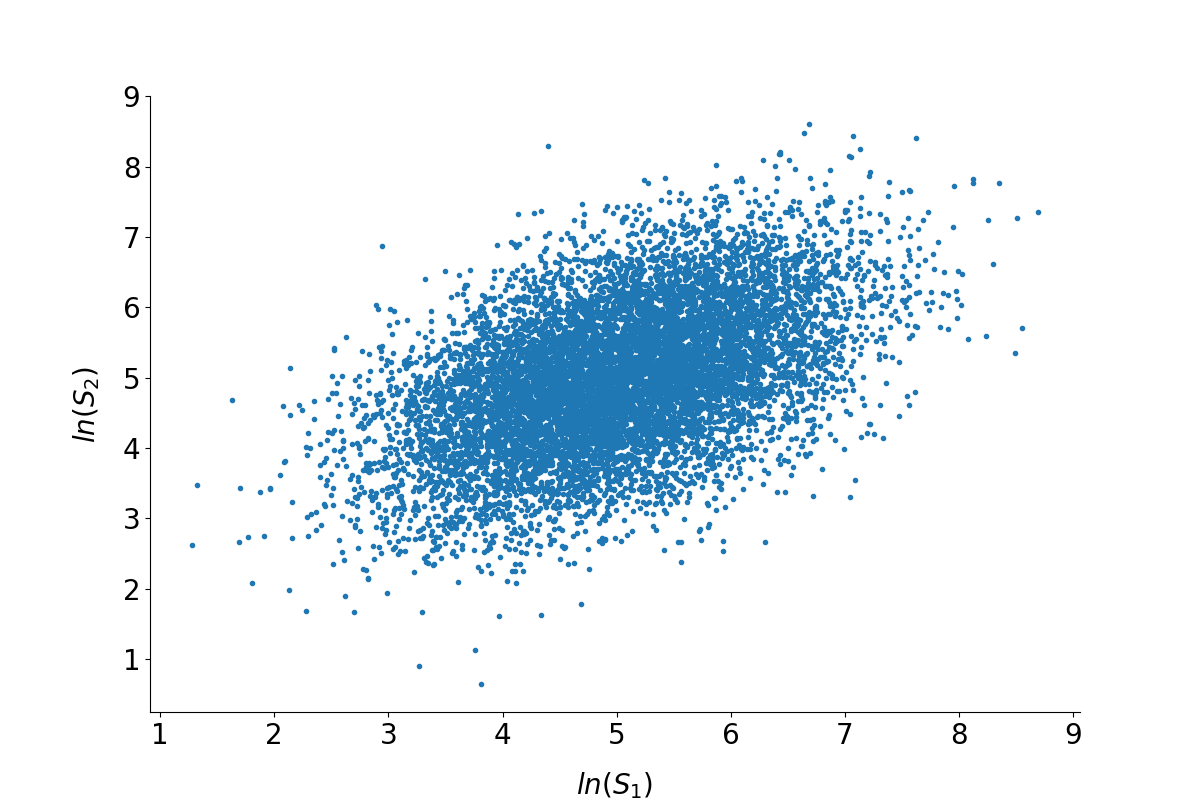
\includegraphics{fig-distribution-skills-latent-joint}}
	\end{figure}
\end{frame}
%-------------------------------------------------------------------------------
%-------------------------------------------------------------------------------
\begin{frame}
	\begin{figure}[htp]\centering
		\caption{Marginal Distribution of Skill}\label{Marginal Distribution of Skill}\scalebox{0.35}{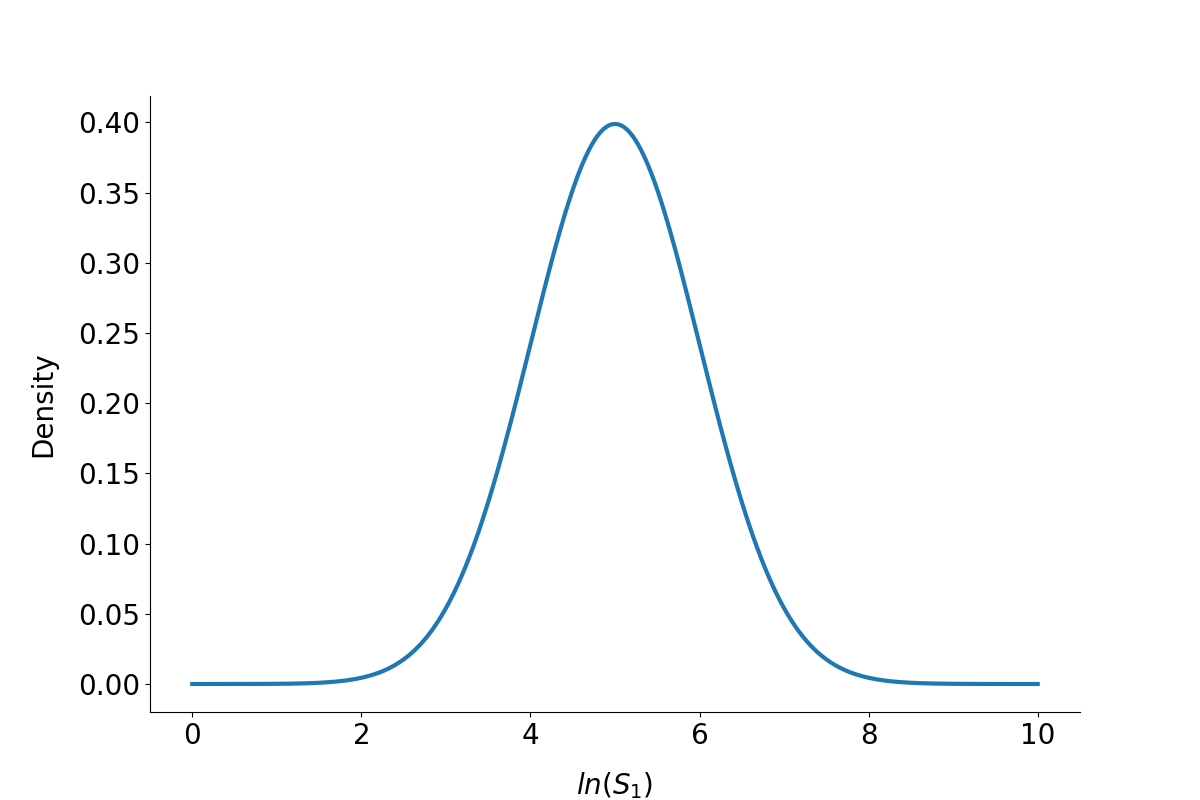
\includegraphics{fig-distribution-skills-latent-marginal}}
	\end{figure}
\end{frame}
%-------------------------------------------------------------------------------
%-------------------------------------------------------------------------------
\begin{frame}
	The proportion of the population working in sector one $P_1$
	\begin{align*}
	P_1 = \int^\infty_0 \int^{\pi_1 s_1 / \pi_2}_0 f(s_1, s_s) ds_1ds_2
	\end{align*}	
	The density of skills employed in sector one differs from the population density of skills.
	\begin{align*}
	f(s_1) & = \int^\infty_0 f(s_1, s_2) ds_2 \\
	g_1(s_1 \mid \pi_1 S_1 > \pi_2 S_2) & = \frac{1}{P_1} \int^{\pi_1 s_1 /\pi_2}_0 f(s_1, s_2) ds_2
	\end{align*}
	The distribution of skills employed in sector 1 differs from the population distribution of skills due to comparative advantage.
\end{frame}
%-------------------------------------------------------------------------------
%-------------------------------------------------------------------------------
\begin{frame}
	\begin{figure}[htp]\centering
		\caption{Latent and Observed Distribution of Skill}\label{Latent and Observed Distribution of Skill}\scalebox{0.35}{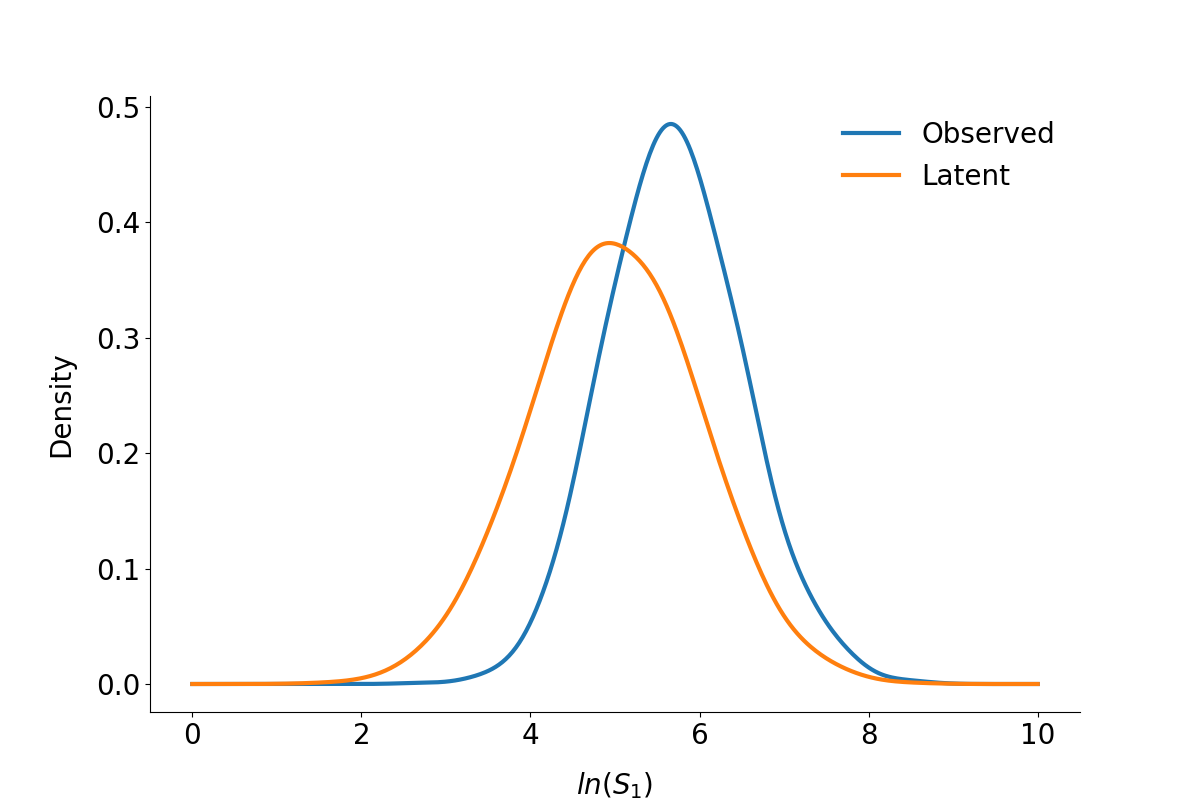
\includegraphics{fig-distribution-skills-both-marginal}}
	\end{figure}
\end{frame}




